% -*- TeX -*- -*- DE -*-

\chapter{PatchCore \cite{patchcore}}\label{ch:PatchCore}
\subsection{Einleitung}
Die Methode \textbf{PatchCore} wurde erstmals am 15. Juni 2021 in Zusammenarbeit der Universität Tübingen und Amazon AWS im Paper \glqq Towards Total \ 
Recall in Industrial Anomaly Detection\grqq{} veröffentlicht. \ 
In seiner zweiten Fassung vom 5. Mai 2022 wurde das Paper bei der Konferenz CVPR 2022 (Computer Vision and Pattern Recognition) akzeptiert und mit \ 
über 290 Zitierungen eines der populärsten Paper im Bereich der Unüberwachten Anomaliedetektion.\\
Die Grundlage dieses Ansatzes sind wiederum \glqq Einbettungen\grqq{} (Embeddings) von Merkmalen (Features), \ 
die aus den Eingabebildern mithilfe eines auf \glqq ImageNet\grqq{} vortrainiertem \glqq Convolutional Neural Network (CNN)\grqq{} erzeugt werden.\
Damit ähnelt sich die Methode PatchCore sowohl SPADE\ref{sec:SPADE}, also auch PaDiM\ref{sec:PaDiM} und greift die in \ref{subsec:ResNetsAsFeatureExtractor} \
beschriebene Vorgehensweise auf.\
Wie wir später sehen werden, unterscheidet sich der Einbettungsprozess jedoch recht deutlich von den bisherigen Methoden.\
% Wie in einigen vorangegangenen Veröffentlichungen im Bereich der Unüberwachten Anomaliedetektion, werden auch hier die Features in \glqq Patches\grqq{} \ 
% unterteilt, um die Lokalität der Anomalien zu erhalten. Diese werden folgend als \textbf{\glqq Patch Features\grqq{}} bezeichnet.\
Weiter wird die eigentliche Anomaliedetektion, wie bereits bei der Methode SPADE mithilfe einer Nächsten Nachbar Suche \ 
(Nearest Neighbor Search; NN) in einer \glqq Memory-Bank \grqq{} durchgeführt.\
Die wesentliche Weitereentwicklung gegenüber SPADE liegt vor allem in der Methode, wie die Memory-Bank aufgebaut wird. Durch die Auswahl möglichst representativer \
Elemente in der Memory Bank, kann die Anzahl der Elemente in der deutlich reduziert werden, was einer Reduzierung der Laufzeit bedeutet.\\
Auch gut 2 Jahre nach Veröffentlichung ist die PatchCore Methode insbesondere auf dem MVTecAD-Datensatz\ref{sec:DatensatzMVTecAD} mit einer Genauigkeit (Auccuracy) \ 
von maximal \num{99,6}\% (\glqq PatchCore Ensemble\grqq{}) absolut konkurrenzfähig und wird in vielen Veröffentlichungen als \glqq State-of-the-Art\grqq{} Methode verwendet.\\
Im Laufe dieses Kapitels soll zunächst die Funktionsweise der Methode PatchCore erläutert werden. Anschließend evaluieren wir die Originalmethode im Hinblick auf Laufzeit und Genauigkeit. \
Im sich dann anschließenden Teil werden zahlreiche Modifikationen besprochen, die versuchen, die Laufzeit auf zu Reduzieren und dabei möglichst viel der Genauigkeit zu erhalten.\

% Zunächst wollen wir die grundsätzliche Funktionsweise der Methode PatchCore erläutern. Anschließend bewerten wir die Methode im Hinblick auf Laufzeit und Genauigkeit. \
% Anschließend werden zahlreiche Adaptionen der Methode vorgestellt, die im Sinne des Ziels dieser Arbeit die Laufzeit der Methode reduzieren und dabei die Genauigkeit möglichst wenig beeinträchtigen sollen.\
\section{Funktionsweise}
\label{sec:Funktionsweise}
unächst kann zwischen zwei Phasen unterschieden werden: Der Trainingsphase und der Testphase.\
In der Trainingsphase werden die \glqq (locally aware) \textbf{Patch Features}\grqq{} aus den Trainingsbildern (\glqq Nominal Samples\grqq{}) extrahiert. \ 
Hierzu wird ein \glqq Pretrained Encoder\grqq{} verwendet, analog zu \ref{subsec:ResNetsAsFeatureExtractor}.\
Anschließend findet eine Unterabtastung bzw. eine Auswahl der Patch Features statt, die in der \glqq Memory Bank\grqq{} gespeichert werden. \ 
Dieser Vorgang wird als \glqq Coreset Subsampling\grqq{} bezeichnet.Ist diese Memory Bank erzeugt, ist die Methode initialisiert und das Training abgeschlossen.\ 
In der Testphase werden die Patch Features auf die gleiche Weise aus den \glqq Test Samples\grqq{} extrahiert, wie in der Trainingsphase. Jedes dieser Patch Features wird nun mit den Patch Features in der Memory Bank verglichen.\ 
Dies geschieht mit einer \glqq Nearest Neighbor Search\grqq{} (NN). Aus den Distanzen zum Nächsten Nachbarn kann dann, wie in \ref{sec:PaDiM} eine räumlich aufgelöste anomaliekarte erzeugt werden.\ 
Auf Grundlage dieser Anomaliekarte geschieht dann die Instanzklassifizierung als nominal oder anomal. Nachfolgende Abbildung \ref{fig:PatchCore}, die aus der Veröffentlichung übernommen wurde, zeigt \ 
die Funktionsweise der Methode PatchCore.\
\begin{figure}[h]
    \centering
    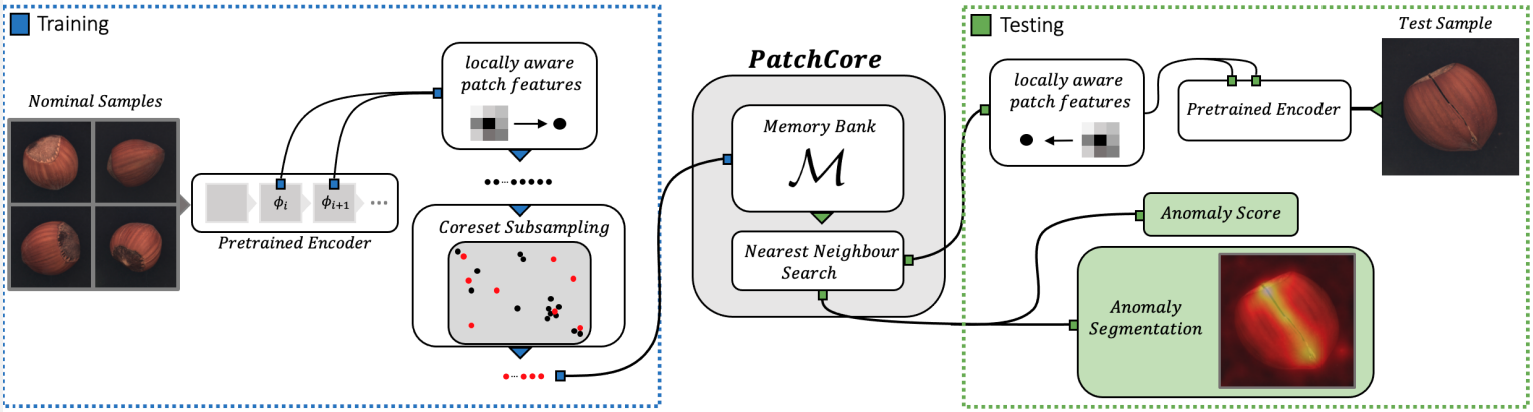
\includegraphics[width=0.95\textwidth]{bilder/patchcore.png}
    \caption{PatchCore}
    \label{fig:PatchCore}
\end{figure}
\subsection{Erzeugen der Patch Features}\label{subsec:ErzeugenDerPatchFeatures}
Zunächst werden einige Notationen definiert, die im Folgenden verwendet werden. Es wird sich dabei auf die Notationen aus der Veröffentlichung bezogen.\
So wird die Menge aller Trainingsbilder als $\mathcal{X}_{train}$ bezeichnet. Die Menge aller Testbilder als $\mathcal{X}_{test}$.\
Für den Trainingsdatensatz gilt im Sinne der Unüberwachtheit, dass es sich um ausschließlich nominale Samples handelt. Im Testdatensatz können sowohl nominale als auch anomale Samples enthalten sein.\
% Werden nominale Samples mit $0$
Bezeichnen wir die wahre Klassenzugehörigkeit eines Bildes $x$ als $y_{x}$, so kann diese entweder $0$ (nominal) oder $1$ (anomal) sein. Für den Trainingsdatensatz gilt dann:\
$\forall x \in \mathcal{X}_{train}: y_{x} = 0$ und für den Testdatensatz $\forall x \in \mathcal{X}_{test}: y_{x} \in \{0,1\}$.\\
Den bereits in \ref{sec:SPADE} und \ref{sec:PaDiM} angetroffenen \glqq Pretrained Encoder\grqq{} wird als $\phi$ bezeichnet.\
Es wird dabei, wie bereits gesehen, nicht der Ausgang dieses Netzwerkes benutzt, sondern die Feature Maps aus einer bestimmten Schicht $j$ des Netzwerkes. \
Im Falle von ResNets, die auch in dieser Veröffentlichung hauptsächlich verwendet werden, ist $j\in \{1,2,3,4\}$.\ 
$j$ wird folgend auch als \glqq Hierarchielevel\grqq{} bezeichnet und spielt eine wichige Rolle.\
$\phi_{i,j} = \phi_{j}(x_{i})$ bezeichnet die Feature Map des Bildes $x_{i}\in \mathcal{X}$ aus dem Hierarchielevel $j$.\
Wie bereits in \ref{subsec:SPADEResults} diskutiert, ist eine sinnvolle Auswahl der Hierarchielevel eine wichtige Voraussetzung für gute Ergebnisse.\
Auch die Autoren von PatchCore weisen auf diese Problemstellung hin. Man könne, wie bei SPADE, die letzte Ebene in der Merkmalshierarchie des Netzes verwenden. \
Dies bringe aber die folgenden zwei Probleme mit sich. Erstens gehe dabei mehr lokalisierte nominale Informationen verloren. Das sei während der Trainingsphase kritisch, \
weil die Arten von Anomalien, die zum Testzeitpunkt auftreten, nicht im Voraus bekannt seien und die möglichst vollständige Erfassung des Normals notwendig sei.\
Zweitens seien die sehr tiefen und abstrakten Merkmale in den vortrainierten ImageNet-Netzwerken auf die Aufgabe der Klassifizierung natürlicher Bilder ausgerichtet, \ 
welche nur wenig direkte Überschneidungen mit der hier vorliegenden Aufgabe der industriellen aufweise. \
Es wird deshalb vorgeschlagen, Merkmale aus den mittleren Hierarchieleveles zu verwenden. Das entspricht bei ResNets $j\in \{2,3\}$.\
Wie in \ref{fig:ResNetPyramid} zu erkennen, handelt es sich bei $\phi_{i,j}$ um einen dreidimensionalen Tensor: $\phi_{i,j}\in \mathbb{R}^{c^{*}\times h^{*}\times w^{*}}$\
mit $c^{*}$ als Tiefe der Feature Maps, $h^{*}$ als Höhe und $w^{*}$ als Breite. \
$\phi_{i,j}(h,w)\in\mathbb{R}^{c^{*}}$ bezeichnet dann den zur Position $h\in\{1,...,h^{*}\}$ und $w\in\{1,...,w^{*}\}$ gehörenden Vektor der Länge $c^{*}$.\
Unter der Annahmen, dass die Größe des Feldes im Originalbild $x_{i}$, das Einfluss auf ein $\phi_{i,j}(h,w)$ nimmt (\glqq Receptive Field\grqq{}), \
ausreichend groß ist, um einen ausreichenden räumlichen Kontext zu erfassen, eignet sich dieser Vektor als \glqq Patch Feature\grqq{} für eine gegenüber \ 
räumlichen Variationen robuste Anomaliedetektion.\\
Um diese wünschenswerte Annahme zu erfüllen, wird eine Aggregation der lokal umliegenden Regionen (\glqq local Neighborhood Aggregation\grqq{}) durchgeführt, das nachfolgend \
vorgestellt wird und die Größe des Receptive Fields steuert.\\
Dafür wird die oben eingeführte Notation für $\phi_{i,j}(h,w)$ um eine ungerade Feldgröße (\glqq patchsize\grqq{}) $p$ erweitert, die die benachbarten Feauture Vektoren \
mit einbezieht. Zunächst wird diese Nachbarschaft wie folgt definiert:\
$$
\mathcal{N}_{p}^{(h,w)} = \{(a,b)| a \in [h-\left\lfloor \frac{p}{2}\right\rfloor,...,h+\left\lfloor \frac{p}{2} \right\rfloor], b \in [w-\left\lfloor \frac{p}{2}\right\rfloor,...,w+\left\lfloor \frac{p}{2}\right\rfloor]\}
$$ 
Damit ergeben sich schließlich die \glqq Patch Features\grqq{} zu\
$$
\phi_{i,j}\Big(\mathcal{N}_{p}^{(h,w)}\Big) = f_{agg}\Big(\{\phi_{i,j}(a,b)| (a,b) \in \mathcal{N}_{p}^{(h,w)}\}\Big),
$$
wobei $f_{agg}$ eine Aggregationsfunktion ist. Die Aggregationsfunktionsfunktion, die in der PatchCore Methode verwendet wird, ist ein adptives \glqq Average Pooling\grqq{}, \
in einer Dimension, die unabhängig von der Länge der Eingangsfeature, immer eine feste Länge $d$ ausgibt.\
%  Hier wird kurz angerissen, was es mit PatchCore auf sich hat. 
% \begin{itemize}
%     \item Popularität, Erscheinungsdatum, Performance, Ersteller, Zitierungen
%     \item Wie funktioniert PatchCore
%     \begin{itemize}
%         \item Training
%         \item Inferenz/Test
%     \end{itemize}
%     \item Implementierung
%     \item Baseline
%     \item Anpassungen
%     \item Fazit
% \end{itemize}
% NUR DER FCK!

\section{Baseline}
\label{sec:Baseline}
Hallo

\section{Adaptionen}
\label{sec:Adaptionen}
Hallo2